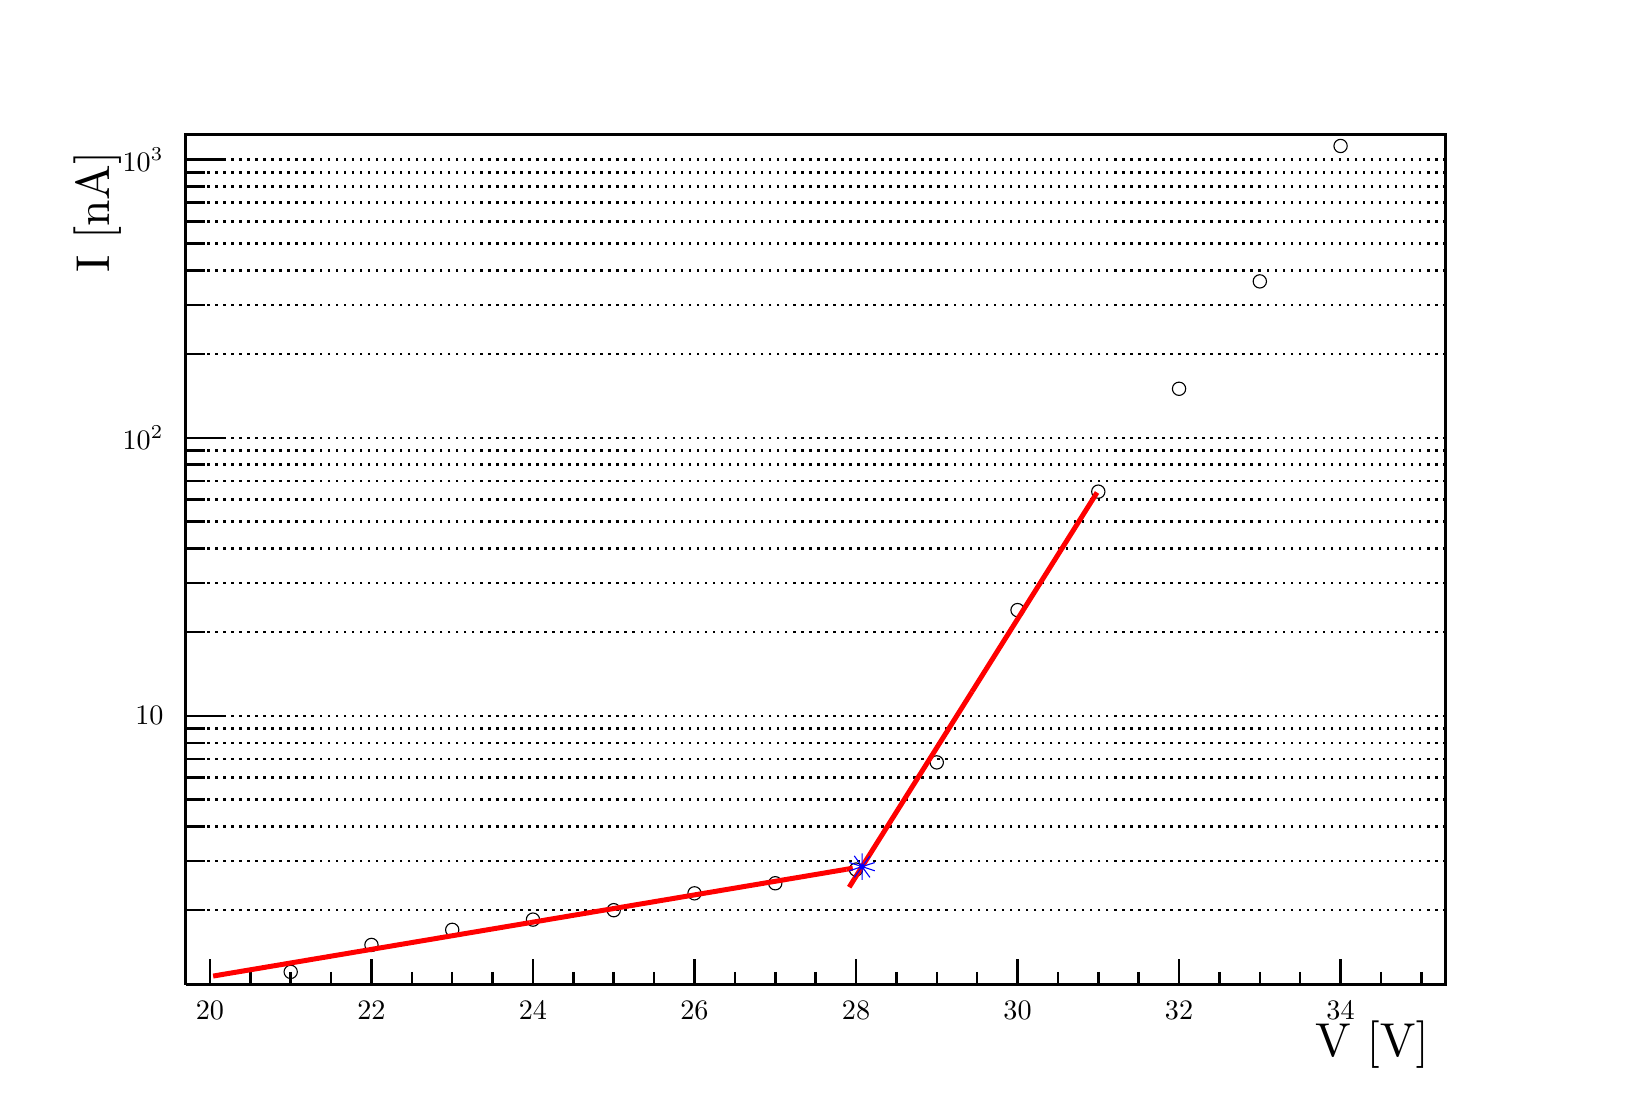
\begin{tikzpicture}
\pgfdeclareplotmark{cross} {
\pgfpathmoveto{\pgfpoint{-0.3\pgfplotmarksize}{\pgfplotmarksize}}
\pgfpathlineto{\pgfpoint{+0.3\pgfplotmarksize}{\pgfplotmarksize}}
\pgfpathlineto{\pgfpoint{+0.3\pgfplotmarksize}{0.3\pgfplotmarksize}}
\pgfpathlineto{\pgfpoint{+1\pgfplotmarksize}{0.3\pgfplotmarksize}}
\pgfpathlineto{\pgfpoint{+1\pgfplotmarksize}{-0.3\pgfplotmarksize}}
\pgfpathlineto{\pgfpoint{+0.3\pgfplotmarksize}{-0.3\pgfplotmarksize}}
\pgfpathlineto{\pgfpoint{+0.3\pgfplotmarksize}{-1.\pgfplotmarksize}}
\pgfpathlineto{\pgfpoint{-0.3\pgfplotmarksize}{-1.\pgfplotmarksize}}
\pgfpathlineto{\pgfpoint{-0.3\pgfplotmarksize}{-0.3\pgfplotmarksize}}
\pgfpathlineto{\pgfpoint{-1.\pgfplotmarksize}{-0.3\pgfplotmarksize}}
\pgfpathlineto{\pgfpoint{-1.\pgfplotmarksize}{0.3\pgfplotmarksize}}
\pgfpathlineto{\pgfpoint{-0.3\pgfplotmarksize}{0.3\pgfplotmarksize}}
\pgfpathclose
\pgfusepathqstroke
}
\pgfdeclareplotmark{cross*} {
\pgfpathmoveto{\pgfpoint{-0.3\pgfplotmarksize}{\pgfplotmarksize}}
\pgfpathlineto{\pgfpoint{+0.3\pgfplotmarksize}{\pgfplotmarksize}}
\pgfpathlineto{\pgfpoint{+0.3\pgfplotmarksize}{0.3\pgfplotmarksize}}
\pgfpathlineto{\pgfpoint{+1\pgfplotmarksize}{0.3\pgfplotmarksize}}
\pgfpathlineto{\pgfpoint{+1\pgfplotmarksize}{-0.3\pgfplotmarksize}}
\pgfpathlineto{\pgfpoint{+0.3\pgfplotmarksize}{-0.3\pgfplotmarksize}}
\pgfpathlineto{\pgfpoint{+0.3\pgfplotmarksize}{-1.\pgfplotmarksize}}
\pgfpathlineto{\pgfpoint{-0.3\pgfplotmarksize}{-1.\pgfplotmarksize}}
\pgfpathlineto{\pgfpoint{-0.3\pgfplotmarksize}{-0.3\pgfplotmarksize}}
\pgfpathlineto{\pgfpoint{-1.\pgfplotmarksize}{-0.3\pgfplotmarksize}}
\pgfpathlineto{\pgfpoint{-1.\pgfplotmarksize}{0.3\pgfplotmarksize}}
\pgfpathlineto{\pgfpoint{-0.3\pgfplotmarksize}{0.3\pgfplotmarksize}}
\pgfpathclose
\pgfusepathqfillstroke
}
\pgfdeclareplotmark{newstar} {
\pgfpathmoveto{\pgfqpoint{0pt}{\pgfplotmarksize}}
\pgfpathlineto{\pgfqpointpolar{44}{0.5\pgfplotmarksize}}
\pgfpathlineto{\pgfqpointpolar{18}{\pgfplotmarksize}}
\pgfpathlineto{\pgfqpointpolar{-20}{0.5\pgfplotmarksize}}
\pgfpathlineto{\pgfqpointpolar{-54}{\pgfplotmarksize}}
\pgfpathlineto{\pgfqpointpolar{-90}{0.5\pgfplotmarksize}}
\pgfpathlineto{\pgfqpointpolar{234}{\pgfplotmarksize}}
\pgfpathlineto{\pgfqpointpolar{198}{0.5\pgfplotmarksize}}
\pgfpathlineto{\pgfqpointpolar{162}{\pgfplotmarksize}}
\pgfpathlineto{\pgfqpointpolar{134}{0.5\pgfplotmarksize}}
\pgfpathclose
\pgfusepathqstroke
}
\pgfdeclareplotmark{newstar*} {
\pgfpathmoveto{\pgfqpoint{0pt}{\pgfplotmarksize}}
\pgfpathlineto{\pgfqpointpolar{44}{0.5\pgfplotmarksize}}
\pgfpathlineto{\pgfqpointpolar{18}{\pgfplotmarksize}}
\pgfpathlineto{\pgfqpointpolar{-20}{0.5\pgfplotmarksize}}
\pgfpathlineto{\pgfqpointpolar{-54}{\pgfplotmarksize}}
\pgfpathlineto{\pgfqpointpolar{-90}{0.5\pgfplotmarksize}}
\pgfpathlineto{\pgfqpointpolar{234}{\pgfplotmarksize}}
\pgfpathlineto{\pgfqpointpolar{198}{0.5\pgfplotmarksize}}
\pgfpathlineto{\pgfqpointpolar{162}{\pgfplotmarksize}}
\pgfpathlineto{\pgfqpointpolar{134}{0.5\pgfplotmarksize}}
\pgfpathclose
\pgfusepathqfillstroke
}
\definecolor{c}{rgb}{1,1,1};
\draw [color=c, fill=c] (0,0) rectangle (20,13.4957);
\draw [color=c, fill=c] (2,1.34957) rectangle (18,12.1461);
\definecolor{c}{rgb}{0,0,0};
\draw [c,line width=0.9] (2,1.34957) -- (2,12.1461) -- (18,12.1461) -- (18,1.34957) -- (2,1.34957);
\definecolor{c}{rgb}{1,1,1};
\draw [color=c, fill=c] (2,1.34957) rectangle (18,12.1461);
\definecolor{c}{rgb}{0,0,0};
\draw [c,line width=0.9] (2,1.34957) -- (2,12.1461) -- (18,12.1461) -- (18,1.34957) -- (2,1.34957);
\draw [c,line width=0.9] (2,1.34957) -- (18,1.34957);
\draw [c,line width=0.9] (2,1.34957) -- (2,12.1461);
\draw [c,dotted,line width=0.9] (18,2.29464) -- (2,2.29464);
\draw [c,dotted,line width=0.9] (18,2.91652) -- (2,2.91652);
\draw [c,dotted,line width=0.9] (18,3.35775) -- (2,3.35775);
\draw [c,dotted,line width=0.9] (18,3.7) -- (2,3.7);
\draw [c,dotted,line width=0.9] (18,3.97963) -- (2,3.97963);
\draw [c,dotted,line width=0.9] (18,4.21606) -- (2,4.21606);
\draw [c,dotted,line width=0.9] (18,4.42087) -- (2,4.42087);
\draw [c,dotted,line width=0.9] (18,4.60152) -- (2,4.60152);
\draw [c,dotted,line width=0.9] (18,4.76311) -- (2,4.76311);
\draw [c,dotted,line width=0.9] (18,5.82623) -- (2,5.82623);
\draw [c,dotted,line width=0.9] (18,6.44811) -- (2,6.44811);
\draw [c,dotted,line width=0.9] (18,6.88934) -- (2,6.88934);
\draw [c,dotted,line width=0.9] (18,7.23158) -- (2,7.23158);
\draw [c,dotted,line width=0.9] (18,7.51122) -- (2,7.51122);
\draw [c,dotted,line width=0.9] (18,7.74765) -- (2,7.74765);
\draw [c,dotted,line width=0.9] (18,7.95245) -- (2,7.95245);
\draw [c,dotted,line width=0.9] (18,8.1331) -- (2,8.1331);
\draw [c,dotted,line width=0.9] (18,8.2947) -- (2,8.2947);
\draw [c,dotted,line width=0.9] (18,9.35781) -- (2,9.35781);
\draw [c,dotted,line width=0.9] (18,9.97969) -- (2,9.97969);
\draw [c,dotted,line width=0.9] (18,10.4209) -- (2,10.4209);
\draw [c,dotted,line width=0.9] (18,10.7632) -- (2,10.7632);
\draw [c,dotted,line width=0.9] (18,11.0428) -- (2,11.0428);
\draw [c,dotted,line width=0.9] (18,11.2792) -- (2,11.2792);
\draw [c,dotted,line width=0.9] (18,11.484) -- (2,11.484);
\draw [c,dotted,line width=0.9] (18,11.6647) -- (2,11.6647);
\draw [c,dotted,line width=0.9] (18,11.8263) -- (2,11.8263);
\draw [c,line width=0.9] (2,1.34957) -- (18,1.34957);
\draw [anchor= east] (18,0.593811) node[scale=1.71821, color=c, rotate=0]{V [V]};
\draw [c,line width=0.9] (2.30769,1.67347) -- (2.30769,1.34957);
\draw [c,line width=0.9] (2.82051,1.51152) -- (2.82051,1.34957);
\draw [c,line width=0.9] (3.33333,1.51152) -- (3.33333,1.34957);
\draw [c,line width=0.9] (3.84615,1.51152) -- (3.84615,1.34957);
\draw [c,line width=0.9] (4.35897,1.67347) -- (4.35897,1.34957);
\draw [c,line width=0.9] (4.8718,1.51152) -- (4.8718,1.34957);
\draw [c,line width=0.9] (5.38462,1.51152) -- (5.38462,1.34957);
\draw [c,line width=0.9] (5.89744,1.51152) -- (5.89744,1.34957);
\draw [c,line width=0.9] (6.41026,1.67347) -- (6.41026,1.34957);
\draw [c,line width=0.9] (6.92308,1.51152) -- (6.92308,1.34957);
\draw [c,line width=0.9] (7.4359,1.51152) -- (7.4359,1.34957);
\draw [c,line width=0.9] (7.94872,1.51152) -- (7.94872,1.34957);
\draw [c,line width=0.9] (8.46154,1.67347) -- (8.46154,1.34957);
\draw [c,line width=0.9] (8.97436,1.51152) -- (8.97436,1.34957);
\draw [c,line width=0.9] (9.48718,1.51152) -- (9.48718,1.34957);
\draw [c,line width=0.9] (10,1.51152) -- (10,1.34957);
\draw [c,line width=0.9] (10.5128,1.67347) -- (10.5128,1.34957);
\draw [c,line width=0.9] (11.0256,1.51152) -- (11.0256,1.34957);
\draw [c,line width=0.9] (11.5385,1.51152) -- (11.5385,1.34957);
\draw [c,line width=0.9] (12.0513,1.51152) -- (12.0513,1.34957);
\draw [c,line width=0.9] (12.5641,1.67347) -- (12.5641,1.34957);
\draw [c,line width=0.9] (13.0769,1.51152) -- (13.0769,1.34957);
\draw [c,line width=0.9] (13.5897,1.51152) -- (13.5897,1.34957);
\draw [c,line width=0.9] (14.1026,1.51152) -- (14.1026,1.34957);
\draw [c,line width=0.9] (14.6154,1.67347) -- (14.6154,1.34957);
\draw [c,line width=0.9] (15.1282,1.51152) -- (15.1282,1.34957);
\draw [c,line width=0.9] (15.641,1.51152) -- (15.641,1.34957);
\draw [c,line width=0.9] (16.1538,1.51152) -- (16.1538,1.34957);
\draw [c,line width=0.9] (16.6667,1.67347) -- (16.6667,1.34957);
\draw [c,line width=0.9] (2.30769,1.67347) -- (2.30769,1.34957);
\draw [c,line width=0.9] (16.6667,1.67347) -- (16.6667,1.34957);
\draw [c,line width=0.9] (17.1795,1.51152) -- (17.1795,1.34957);
\draw [c,line width=0.9] (17.6923,1.51152) -- (17.6923,1.34957);
\draw [anchor=base] (2.30769,0.904212) node[scale=1.01821, color=c, rotate=0]{20};
\draw [anchor=base] (4.35897,0.904212) node[scale=1.01821, color=c, rotate=0]{22};
\draw [anchor=base] (6.41026,0.904212) node[scale=1.01821, color=c, rotate=0]{24};
\draw [anchor=base] (8.46154,0.904212) node[scale=1.01821, color=c, rotate=0]{26};
\draw [anchor=base] (10.5128,0.904212) node[scale=1.01821, color=c, rotate=0]{28};
\draw [anchor=base] (12.5641,0.904212) node[scale=1.01821, color=c, rotate=0]{30};
\draw [anchor=base] (14.6154,0.904212) node[scale=1.01821, color=c, rotate=0]{32};
\draw [anchor=base] (16.6667,0.904212) node[scale=1.01821, color=c, rotate=0]{34};
\draw [c,line width=0.9] (2,1.34957) -- (2,12.1461);
\draw [anchor= east] (0.88,12.1461) node[scale=1.71821, color=c, rotate=90]{I [nA]};
\draw [c,line width=0.9] (2.24,2.29464) -- (2,2.29464);
\draw [c,line width=0.9] (2.24,2.91652) -- (2,2.91652);
\draw [c,line width=0.9] (2.24,3.35775) -- (2,3.35775);
\draw [c,line width=0.9] (2.24,3.7) -- (2,3.7);
\draw [c,line width=0.9] (2.24,3.97963) -- (2,3.97963);
\draw [c,line width=0.9] (2.24,4.21606) -- (2,4.21606);
\draw [c,line width=0.9] (2.24,4.42087) -- (2,4.42087);
\draw [c,line width=0.9] (2.24,4.60152) -- (2,4.60152);
\draw [c,line width=0.9] (2.48,4.76311) -- (2,4.76311);
\draw [anchor= east] (1.844,4.76311) node[scale=1.01821, color=c, rotate=0]{10};
\draw [c,line width=0.9] (2.24,5.82623) -- (2,5.82623);
\draw [c,line width=0.9] (2.24,6.44811) -- (2,6.44811);
\draw [c,line width=0.9] (2.24,6.88934) -- (2,6.88934);
\draw [c,line width=0.9] (2.24,7.23158) -- (2,7.23158);
\draw [c,line width=0.9] (2.24,7.51122) -- (2,7.51122);
\draw [c,line width=0.9] (2.24,7.74765) -- (2,7.74765);
\draw [c,line width=0.9] (2.24,7.95245) -- (2,7.95245);
\draw [c,line width=0.9] (2.24,8.1331) -- (2,8.1331);
\draw [c,line width=0.9] (2.48,8.2947) -- (2,8.2947);
\draw [anchor= east] (1.844,8.2947) node[scale=1.01821, color=c, rotate=0]{$10^{2}$};
\draw [c,line width=0.9] (2.24,9.35781) -- (2,9.35781);
\draw [c,line width=0.9] (2.24,9.97969) -- (2,9.97969);
\draw [c,line width=0.9] (2.24,10.4209) -- (2,10.4209);
\draw [c,line width=0.9] (2.24,10.7632) -- (2,10.7632);
\draw [c,line width=0.9] (2.24,11.0428) -- (2,11.0428);
\draw [c,line width=0.9] (2.24,11.2792) -- (2,11.2792);
\draw [c,line width=0.9] (2.24,11.484) -- (2,11.484);
\draw [c,line width=0.9] (2.24,11.6647) -- (2,11.6647);
\draw [c,line width=0.9] (2.48,11.8263) -- (2,11.8263);
\draw [anchor= east] (1.844,11.8263) node[scale=1.01821, color=c, rotate=0]{$10^{3}$};
\foreach \P in {(3.33333,1.51117), (4.35897,1.85341), (5.38462,2.04538), (6.41026,2.17507), (7.4359,2.29464), (8.46154,2.509), (9.48718,2.63689), (10.5128,2.81071), (11.5385,4.17161), (12.5641,6.10586), (13.5897,7.61021), (14.6154,8.91658),
 (15.641,10.2805), (16.6667,12.0001)}{\draw[mark options={color=c,fill=c},mark size=2.402402pt,mark=o] plot coordinates {\P};}
\definecolor{c}{rgb}{1,0,0};
\draw [c,line width=1.8] (2.34872,1.45835) -- (2.43077,1.47218) -- (2.51282,1.48601) -- (2.59487,1.49985) -- (2.67692,1.51368) -- (2.75897,1.52751) -- (2.84103,1.54134) -- (2.92308,1.55518) -- (3.00513,1.56901) -- (3.08718,1.58284) --
 (3.16923,1.59668) -- (3.25128,1.61051) -- (3.33333,1.62434) -- (3.41538,1.63818) -- (3.49744,1.65201) -- (3.57949,1.66584) -- (3.66154,1.67967) -- (3.74359,1.69351) -- (3.82564,1.70734) -- (3.90769,1.72117) -- (3.98974,1.73501) -- (4.07179,1.74884)
 -- (4.15385,1.76267) -- (4.2359,1.7765) -- (4.31795,1.79034) -- (4.4,1.80417) -- (4.48205,1.818) -- (4.5641,1.83184) -- (4.64615,1.84567) -- (4.72821,1.8595) -- (4.81026,1.87334) -- (4.89231,1.88717) -- (4.97436,1.901) -- (5.05641,1.91483) --
 (5.13846,1.92867) -- (5.22051,1.9425) -- (5.30256,1.95633) -- (5.38462,1.97017) -- (5.46667,1.984) -- (5.54872,1.99783) -- (5.63077,2.01167) -- (5.71282,2.0255) -- (5.79487,2.03933) -- (5.87692,2.05316) -- (5.95897,2.067) -- (6.04103,2.08083) --
 (6.12308,2.09466) -- (6.20513,2.1085) -- (6.28718,2.12233) -- (6.36923,2.13616);
\draw [c,line width=1.8] (6.36923,2.13616) -- (6.45128,2.14999) -- (6.53333,2.16383) -- (6.61538,2.17766) -- (6.69744,2.19149) -- (6.77949,2.20533) -- (6.86154,2.21916) -- (6.94359,2.23299) -- (7.02564,2.24683) -- (7.10769,2.26066) --
 (7.18974,2.27449) -- (7.27179,2.28832) -- (7.35385,2.30216) -- (7.4359,2.31599) -- (7.51795,2.32982) -- (7.6,2.34366) -- (7.68205,2.35749) -- (7.7641,2.37132) -- (7.84615,2.38516) -- (7.92821,2.39899) -- (8.01026,2.41282) -- (8.09231,2.42665) --
 (8.17436,2.44049) -- (8.25641,2.45432) -- (8.33846,2.46815) -- (8.42051,2.48199) -- (8.50256,2.49582) -- (8.58462,2.50965) -- (8.66667,2.52348) -- (8.74872,2.53732) -- (8.83077,2.55115) -- (8.91282,2.56498) -- (8.99487,2.57882) -- (9.07692,2.59265)
 -- (9.15897,2.60648) -- (9.24103,2.62032) -- (9.32308,2.63415) -- (9.40513,2.64798) -- (9.48718,2.66181) -- (9.56923,2.67565) -- (9.65128,2.68948) -- (9.73333,2.70331) -- (9.81538,2.71715) -- (9.89744,2.73098) -- (9.97949,2.74481) --
 (10.0615,2.75865) -- (10.1436,2.77248) -- (10.2256,2.78631) -- (10.3077,2.80014) -- (10.3897,2.81398);
\draw [c,line width=1.8] (10.3897,2.81398) -- (10.4718,2.82781);
\draw [c,line width=1.8] (10.4262,2.58667) -- (10.4579,2.6373) -- (10.4897,2.68793) -- (10.5215,2.73857) -- (10.5533,2.7892) -- (10.5851,2.83983) -- (10.6169,2.89046) -- (10.6487,2.94109) -- (10.6805,2.99172) -- (10.7123,3.04235) -- (10.7441,3.09299)
 -- (10.7759,3.14362) -- (10.8077,3.19425) -- (10.8395,3.24488) -- (10.8713,3.29551) -- (10.9031,3.34614) -- (10.9349,3.39678) -- (10.9667,3.44741) -- (10.9985,3.49804) -- (11.0303,3.54867) -- (11.0621,3.5993) -- (11.0938,3.64993) --
 (11.1256,3.70056) -- (11.1574,3.7512) -- (11.1892,3.80183) -- (11.221,3.85246) -- (11.2528,3.90309) -- (11.2846,3.95372) -- (11.3164,4.00435) -- (11.3482,4.05499) -- (11.38,4.10562) -- (11.4118,4.15625) -- (11.4436,4.20688) -- (11.4754,4.25751) --
 (11.5072,4.30814) -- (11.539,4.35877) -- (11.5708,4.40941) -- (11.6026,4.46004) -- (11.6344,4.51067) -- (11.6662,4.5613) -- (11.6979,4.61193) -- (11.7297,4.66256) -- (11.7615,4.7132) -- (11.7933,4.76383) -- (11.8251,4.81446) -- (11.8569,4.86509) --
 (11.8887,4.91572) -- (11.9205,4.96635) -- (11.9523,5.01698) -- (11.9841,5.06762);
\draw [c,line width=1.8] (11.9841,5.06762) -- (12.0159,5.11825) -- (12.0477,5.16888) -- (12.0795,5.21951) -- (12.1113,5.27014) -- (12.1431,5.32077) -- (12.1749,5.37141) -- (12.2067,5.42204) -- (12.2385,5.47267) -- (12.2703,5.5233) --
 (12.3021,5.57393) -- (12.3338,5.62456) -- (12.3656,5.67519) -- (12.3974,5.72583) -- (12.4292,5.77646) -- (12.461,5.82709) -- (12.4928,5.87772) -- (12.5246,5.92835) -- (12.5564,5.97898) -- (12.5882,6.02962) -- (12.62,6.08025) -- (12.6518,6.13088) --
 (12.6836,6.18151) -- (12.7154,6.23214) -- (12.7472,6.28277) -- (12.779,6.3334) -- (12.8108,6.38404) -- (12.8426,6.43467) -- (12.8744,6.4853) -- (12.9062,6.53593) -- (12.9379,6.58656) -- (12.9697,6.63719) -- (13.0015,6.68783) -- (13.0333,6.73846) --
 (13.0651,6.78909) -- (13.0969,6.83972) -- (13.1287,6.89035) -- (13.1605,6.94098) -- (13.1923,6.99161) -- (13.2241,7.04225) -- (13.2559,7.09288) -- (13.2877,7.14351) -- (13.3195,7.19414) -- (13.3513,7.24477) -- (13.3831,7.2954) -- (13.4149,7.34604)
 -- (13.4467,7.39667) -- (13.4785,7.4473) -- (13.5103,7.49793) -- (13.5421,7.54856);
\draw [c,line width=1.8] (13.5421,7.54856) -- (13.5738,7.59919);
\definecolor{c}{rgb}{0,0,1};
\foreach \P in {(10.5901,2.84776)}{\draw[mark options={color=c,fill=c},mark size=4.804805pt,mark=10-pointed star] plot coordinates {\P};}
\end{tikzpicture}
